\section*{The Particle in a Box\sectionmark{The Particle in a Box}}

	\begin{questions}
	
		\question Consider a particle in the following one-dimensional ``particle in a box'' potential:
		
			\vspace{0.1in}
			\centerline{
				\begin{minipage}{0.5\textwidth}
					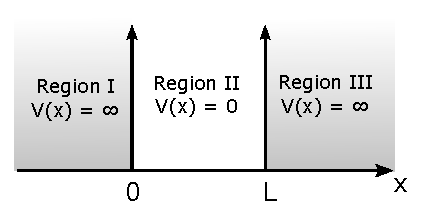
\includegraphics[width=\textwidth]{includes/PIB-FIGURES/PIB}
				\end{minipage}
				\begin{minipage}{0.3\textwidth}
					\begin{equation}
				 		V(x)=\begin{cases}\infty & x<0 \\ 0 & 0 \leq x \leq L \\ \infty & x>L \end{cases} \nonumber
					\end{equation}
				\end{minipage}
		}\vspace{0.1in}
		
			\begin{parts}
			
				\part What is the Hamiltonian in Region II, where $V(x) = 0$?
				
					\begin{equation*}
						\hat H = \answerbox{75}
					\end{equation*}
				
				\part Show that $\Psi(x) = A\cos(kx) + B\sin(kx)$ is an eigenfunction of this Hamiltonian $\hat H$.  What is its eigenvalue?
				
					\begin{solution}[2.75in]
					\end{solution}
				
				\part Set this eigenvalue equal to the energy, $E$. What is $E$ in terms of $k$?
				
					\begin{solution}[1.75in]
					\end{solution}
					
			\end{parts}
			
			\contdnewpg 
			
			\question
				\begin{parts}
			
				\part It is physically impossible for the particle to be in the regions where $V(x) = \infty$, so the probability of finding the particle in these regions has to be zero. 
				
				What does this tell you about the value of the wavefunction in Regions I and III?
					\begin{align*}
						\Psi_{I}(x) = \answerbox{40} & & \Psi_{III}(x) = \answerbox{40}
					\end{align*}
				
				\part The wavefunction must be continuous at every value of $x$.  What does that mean must be true about the value of $\Psi_{II}(x)$ at the edges of the box?
					\begin{align*}
						\Psi_{II}(0) = \answerbox{40} & & \Psi_{II}(L) = \answerbox{40}
					\end{align*}
					
				\part Using the wavefunction $\Psi_{II}(x) = A\cos(kx) + B\sin(kx)$, calculate $\Psi_{II}(0)$ and set it equal to the value you found above. What does this tell you about the value of $A$?
				
					\begin{solution}[2in]
					\end{solution}
				
				\part Now, calculate $\Psi_{II}(L)$. What has to be true about $kL$ in order for $\Psi_{II}(L)$ to equal what you found in part (b)? What does this result tell you about the values of the energy $E$?
				
					\begin{solution}[1.75in]
					\end{solution}
		
			\end{parts}
	\end{questions}

